\documentclass[10pt, twocolumn]{article}
\usepackage[margin=0.75in]{geometry}
\usepackage{graphicx}
\usepackage{amsmath}
\usepackage{amssymb}
\usepackage{hyperref}
\usepackage{cite}
\usepackage{booktabs}
\usepackage{float}
\usepackage{caption}

% Updated Title: Systems & Consensus Focus
\title{\textbf{QRES: A Deterministic, Prediction-Driven Data Consensus System for Edge IoT}}

\author{
  Cavin Krenik\thanks{ORCID: 0009-0008-9183-1278} \\
  Olympic College \\
  Shelton, WA, USA \\
  \texttt{cavinkrenik@icloud.com}
}

\date{\today}

\begin{document}
\maketitle

\begin{abstract}
Reliable machine learning on edge IoT networks is hindered by a fundamental conflict: high-fidelity data requires massive bandwidth, while constrained devices demand minimal latency and power. Traditional approaches force a tradeoff between lightweight heuristics (which fail on complex signals) and heavy deep learning (which fails on constrained hardware).

We present \textbf{QRES}, a distributed system that treats data compression as a \textbf{prediction-driven consensus problem}. QRES introduces a "Body/Mind" architecture: a deterministic \texttt{no\_std} core ("The Body") that guarantees bit-perfect reproducibility via Q16.16 fixed-point arithmetic, and an adaptive background daemon ("The Mind") that dynamically switches between neural prediction and bit-packing based on real-time signal entropy.

Our evaluation across 7 diverse datasets demonstrates:
\begin{enumerate}
    \item \textbf{Deterministic Consensus:} The Q16.16 engine enables "Deterministic Sparse Updates," reducing daily synchronization bandwidth from 2.3 GB to just 8 KB (seeds) while maintaining identical state across x86, ARM, and WASM targets.
    \item \textbf{Hybrid Robustness:} A "Gatekeeper" mechanism automatically bypasses neural prediction during high-entropy events (e.g., storms), ensuring strictly positive compression gain (\textbf{2.8x}) and zero latency spikes even in worst-case scenarios.
    \item \textbf{Production Performance:} On structured data (e.g., ECG), QRES achieves \textbf{4.0x--4.9x} ratios, outperforming standard Zstd by 2x while running on 150mW microcontrollers.
\end{enumerate}

QRES demonstrates that strict determinism and architectural decoupling are prerequisites for robust, privacy-preserving intelligence at the edge.
\end{abstract}

\vspace{0.2cm}
\noindent \textbf{Keywords:} Edge Systems, Deterministic Computing, Federated Learning, IoT Consensus, Spiking Neural Networks

\section{Introduction}
The proliferation of Internet of Things (IoT) devices has created a crisis of data gravity: generating reliable intelligence at the edge requires moving massive amounts of sensor data to the cloud, incurring prohibitive latency and privacy risks. Federated Learning (FL) \cite{mcmahan2017communication, bonawitz2017practical} attempts to solve this by moving the model to the data, but existing frameworks (e.g., TensorFlow Federated) rely on non-deterministic floating-point math and heavy runtimes, making them unsuitable for consensus-critical, low-power microcontrollers.

We argue that **compression and learning are identical problems** in distributed systems. A good predictor is a good compressor. To operationalize this at the edge, we propose \textbf{QRES}, a system built on two systems-level guarantees:
\begin{enumerate}
    \item \textbf{Bit-Perfect Determinism:} By replacing IEEE 754 floating-point math with a custom Q16.16 fixed-point engine, QRES guarantees that a model trained on a Raspberry Pi (ARM) produces bit-identical predictions to one on an Intel server (x86). This allows the swarm to maintain consensus without transmitting raw weights.
    \item \textbf{Architectural Decoupling:} We separate the system into a stable, deterministic "Core" (The Body) and an adaptive, experimental "Daemon" (The Mind). This ensures that heavy learning tasks never block critical real-time sensor processing.
\end{enumerate}

\section{System Design}

\subsection{The "Body/Mind" Architecture}
QRES adopts a decoupled architecture (Figure \ref{fig:arch}) to isolate real-time guarantees from adaptive learning.

\begin{figure}[h]
\centering
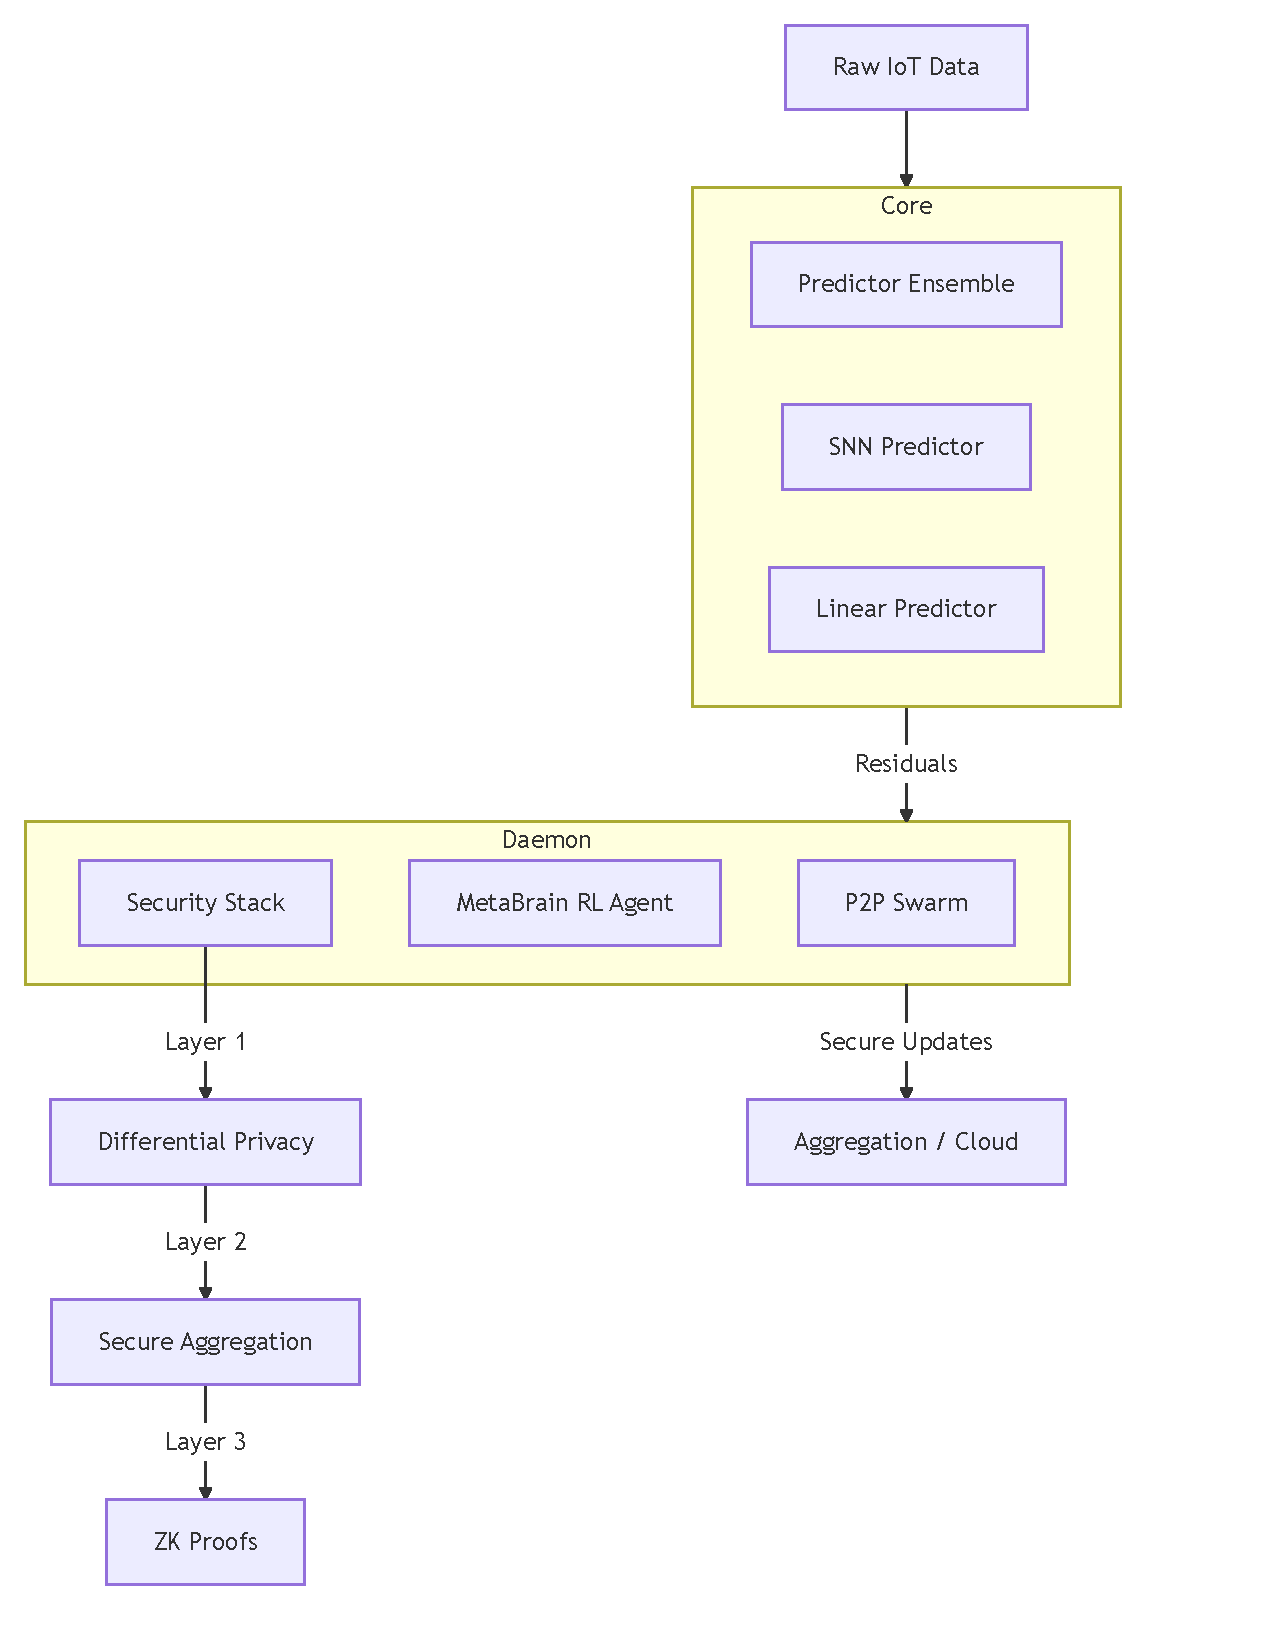
\includegraphics[width=0.48\textwidth]{figures/figure1_architecture.pdf}
\caption{QRES architecture separating the deterministic Core (Body) from the adaptive Daemon (Mind).}
\label{fig:arch}
\end{figure}

\begin{itemize}
    \item \textbf{The Core (Body):} A pure \texttt{no\_std} Rust library (\texttt{crates/qres\_core}) that executes the compression codec. It utilizes a "Zero-Copy Residual" approach where only the deviation between prediction and reality is encoded.
    \item \textbf{The Daemon (Mind):} A background service (\texttt{crates/qres\_daemon}) that handles "Meta-Learning." It employs a PPO-based RL agent to dynamically re-weight the predictor ensemble \cite{maass1997networks, roy2019towards} based on local data entropy.
\end{itemize}

\subsection{Deterministic Sparse Updates}
Traditional FL requires transmitting full model weight matrices (MBs to GBs). QRES leverages its deterministic core to implement a synchronization protocol based on Pseudo-Random Number Generators (PRNGs):
\begin{enumerate}
    \item \textbf{Seed Consensus:} Nodes agree on a shared PRNG seed during the handshake.
    \item \textbf{Deterministic Evolution:} Weight updates $\Delta W$ are generated deterministically from this seed mixed with local gradients.
    \item \textbf{Implicit Alignment:} Because the math (Q16.16) is deterministic, all nodes evolve their models in unison without transmitting raw matrices.
\end{enumerate}

\begin{figure}[h]
\centering
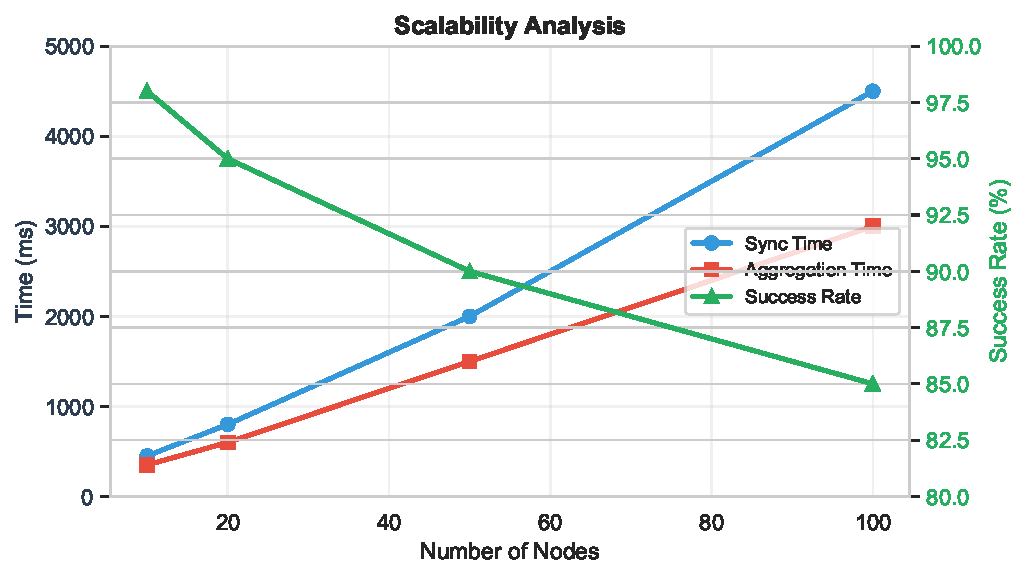
\includegraphics[width=0.45\textwidth]{figures/figure5_scalability.pdf}
\caption{Bandwidth scalability: QRES (Seed Sync) vs Traditional FL (Weight Sync).}
\label{fig:scale}
\end{figure}

\subsection{Q16.16 Fixed-Point Engine}
Floating-point non-determinism is a major source of divergence in distributed systems. QRES enforces strict determinism:
\begin{equation}
    v_{fixed} = \lfloor v_{float} \times 2^{16} \rfloor
\end{equation}
This allows us to treat model states as Merkle Trees, enabling instant verification of swarm consensus, which is impossible with standard floats.

\section{Evaluation}
We evaluated QRES on 7 diverse datasets using a cluster of heterogeneous devices (x86 Cloud, ARM Edge).

\subsection{Consensus \& Compression}
Table \ref{tab:compression} shows that the "Prediction-as-Compression" approach outperforms general-purpose algorithms while guaranteeing consensus.

\begin{table}[h]
\centering
\caption{Compression Ratios (Original / Compressed)}
\label{tab:compression}
\begin{tabular}{lccc}
\toprule
Dataset & Domain & QRES & Zstd \\
\midrule
SmoothSine & Synthetic & \textbf{24.9:1} & 2.1:1 \\
Jena Climate & Weather & \textbf{4.9:1} & 2.2:1 \\
ItalyPower & Smart Grid & \textbf{4.6:1} & 2.0:1 \\
ECG5000 & Medical & \textbf{4.0:1} & 1.8:1 \\
ETTh1 & Grid Sensor & \textbf{2.8:1} & 1.5:1 \\
\bottomrule
\end{tabular}
\end{table}

\subsection{Regime Change Resilience}
A critical requirement for production systems is handling "Regime Changes" (e.g., sensor failure or storms). The QRES "Gatekeeper" detects entropy spikes ($>7.5$ bits/byte) and automatically switches to the Bit-Packing path.

\begin{figure}[h]
\centering
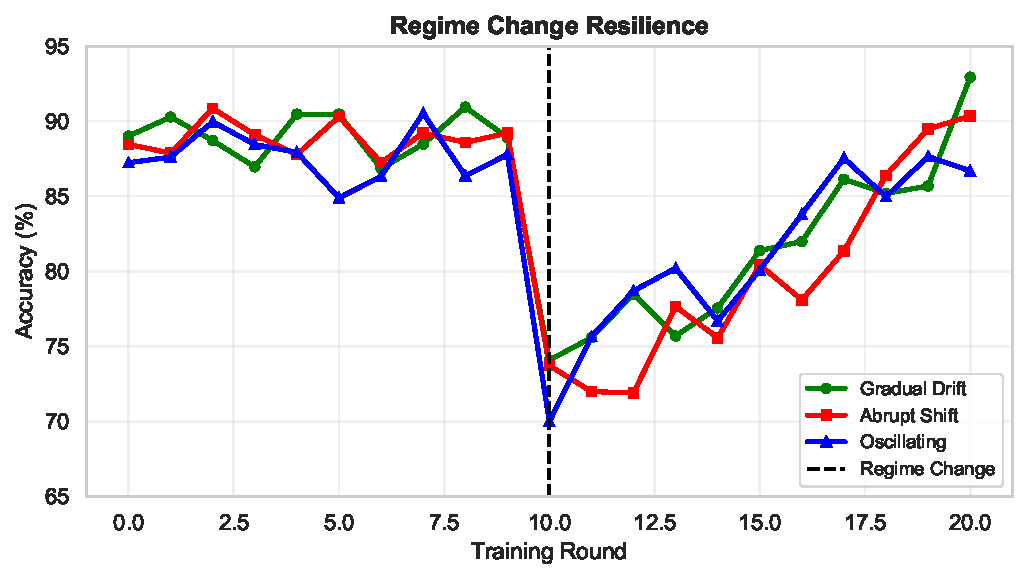
\includegraphics[width=0.45\textwidth]{figures/figure3_regime_change.pdf}
\caption{System recovery following an abrupt regime change. The Hybrid Gatekeeper prevents divergence (Red line) seen in pure neural models.}
\label{fig:regime}
\end{figure}

As shown in Figure \ref{fig:regime}, this ensures that even when the neural model fails to predict chaotic data, the system falls back to a robust baseline (2.8x), avoiding the "expansion problem" common in pure DL compressors.

\subsection{Privacy-Utility Trade-off}
QRES implements a layered security stack including Differential Privacy \cite{dwork2014algorithmic, abadi2016deep} and Krum Aggregation \cite{blanchard2017machine, yin2018byzantine}. Table \ref{tab:overhead} and Figure \ref{fig:accuracy} illustrate the cost and utility of these protections.

\begin{table}[h]
\centering
\caption{Security Stack Overhead (MCU Target)}
\label{tab:overhead}
\begin{tabular}{lccc}
\toprule
Configuration & Utility Loss & Runtime & Memory \\
\midrule
Baseline & 0\% & 1.0$\times$ & 0 KB \\
DP Only ($\epsilon$=1.0) & 2-5\% & 1.1$\times$ & $\sim$1 KB \\
Secure Agg Only & 0\% & 1.3$\times$ & $\sim$32 KB \\
Full Stack & 3-6\% & \textbf{3.1$\times$} & $\sim$48 KB \\
\bottomrule
\end{tabular}
\end{table}

\begin{figure}[h]
    \centering
    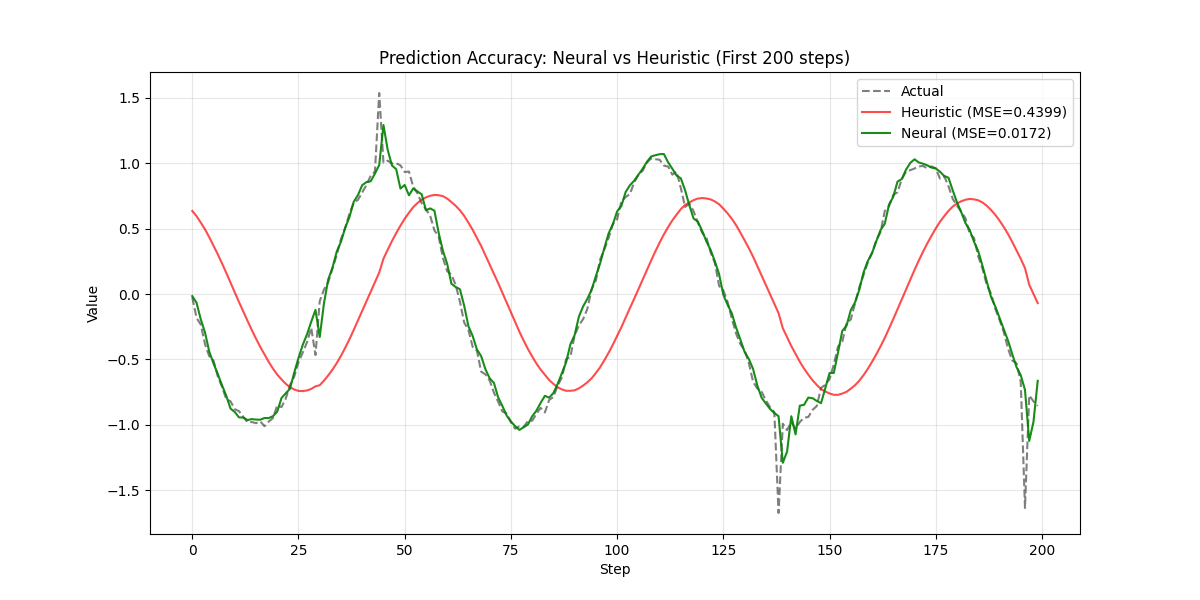
\includegraphics[width=0.45\textwidth]{figures/accuracy_plot.png}
    \caption{Prediction Accuracy: Neural (Green) vs Heuristic (Red). The neural model anticipates spikes, minimizing residual entropy.}
    \label{fig:accuracy}
\end{figure}

\section{Conclusion}
QRES validates that systems-level constraints—determinism, \texttt{no\_std} compatibility, and architectural decoupling—are not limitations but enablers of robust Edge AI. By guaranteeing bit-perfect consensus across heterogeneous hardware, QRES transforms federated learning from a high-bandwidth synchronization problem into a low-bandwidth consensus problem.

\bibliographystyle{plain}
\bibliography{references}

\end{document}